% \documentclass[handout]{beamer}
\documentclass{beamer}

\mode<presentation>
{
  \usetheme{ANLBlue}
  % \usefonttheme[onlymath]{serif}
  % \usetheme{Singapore}
  % \usetheme{Warsaw}
  % \usetheme{Malmoe}
  % \useinnertheme{circles}
  % \useoutertheme{infolines}
  % \useinnertheme{rounded}

  \setbeamercovered{transparent=20}
}

\usepackage[english]{babel}
\usepackage[latin1]{inputenc}
\usepackage{alltt,listings,multirow,ulem,siunitx}
\usepackage[absolute,overlay]{textpos}
\TPGrid{1}{1}
\usepackage{pdfpages}
\usepackage{ulem}
\usepackage{multimedia}
\usepackage{multicol}
\newcommand\hmmax{0}
\newcommand\bmmax{0}
\usepackage{bm}
\usepackage{comment}
\usepackage{subcaption}

% font definitions, try \usepackage{ae} instead of the following
% three lines if you don't like this look
\usepackage{mathptmx}
\usepackage[scaled=.90]{helvet}
% \usepackage{courier}
\usepackage[T1]{fontenc}
\usepackage{tikz}
\usetikzlibrary{decorations.pathreplacing}
\usetikzlibrary{shadows,arrows,shapes.misc,shapes.arrows,shapes.multipart,arrows,decorations.pathmorphing,backgrounds,positioning,fit,petri,calc,shadows,chains,matrix}

\newcommand\vvec{\bm v}
\newcommand\bvec{\bm b}
\newcommand\bxk{\bvec_0 \times \kappa_0 \cdot \nabla}
\newcommand\delp{\nabla_\perp}

% \usepackage{pgfpages}
% \pgfpagesuselayout{4 on 1}[a4paper,landscape,border shrink=5mm]

\usepackage{JedMacros}

\newcommand{\timeR}{t_{\mathrm{R}}}
\newcommand{\timeW}{t_{\mathrm{W}}}
\newcommand{\mglevel}{\ensuremath{\ell}}
\newcommand{\mglevelcp}{\ensuremath{\mglevel_{\mathrm{cp}}}}
\newcommand{\mglevelcoarse}{\ensuremath{\mglevel_{\mathrm{coarse}}}}
\newcommand{\mglevelfine}{\ensuremath{\mglevel_{\mathrm{fine}}}}

%solution and residual
\newcommand{\vx}{\ensuremath{x}}
\newcommand{\vc}{\ensuremath{\hat{x}}}
\newcommand{\vr}{\ensuremath{r}}
\newcommand{\vb}{\ensuremath{b}}

%operators
\newcommand{\vA}{\ensuremath{A}}
\newcommand{\vP}{\ensuremath{I_H^h}}
\newcommand{\vS}{\ensuremath{S}}
\newcommand{\vR}{\ensuremath{I_h^H}}
\newcommand{\vI}{\ensuremath{\hat I_h^H}}
\newcommand{\vV}{\ensuremath{\mathbf{V}}}
\newcommand{\vF}{\ensuremath{F}}
\newcommand{\vtau}{\ensuremath{\mathbf{\tau}}}


\title{Multigrid on the outside: restructuring time integration and adaptivity}
\author{{\bf Jed Brown} \texttt{jedbrown@mcs.anl.gov} (ANL and CU Boulder) \\
  Collaborators in this work: \\
  \quad Debojyoti Ghosh (ANL), Mark Adams (LBL), Matt Knepley (UChicago)
}

% - Use the \inst command only if there are several affiliations.
% - Keep it simple, no one is interested in your street address.
% \institute
% {
%   Mathematics and Computer Science Division \\ Argonne National Laboratory
% }

\date{Berkeley Lab, 2014-01-16}

% This is only inserted into the PDF information catalog. Can be left
% out.
\subject{Talks}


% If you have a file called "university-logo-filename.xxx", where xxx
% is a graphic format that can be processed by latex or pdflatex,
% resp., then you can add a logo as follows:

% \pgfdeclareimage[height=0.5cm]{university-logo}{university-logo-filename}
% \logo{\pgfuseimage{university-logo}}



% Delete this, if you do not want the table of contents to pop up at
% the beginning of each subsection:
% \AtBeginSubsection[]
% {
% \begin{frame}<beamer>
%   \frametitle{Outline}
%   \tableofcontents[currentsection,currentsubsection]
% \end{frame}
% }

\AtBeginSection[]
{
  \begin{frame}<beamer>
    \frametitle{Outline}
    \tableofcontents[currentsection]
  \end{frame}
}

% If you wish to uncover everything in a step-wise fashion, uncomment
% the following command:

% \beamerdefaultoverlayspecification{<+->}

\begin{document}
\lstset{language=C}
\normalem

\begin{frame}
  \titlepage
\end{frame}

\section{Fast solvers for Implicit Runge-Kutta}

\subsection{The memory bandwidth problem}
\begin{frame}{Hardware Arithmetic Intensity}
  \begin{tabular}{lc}
    \toprule
    Operation                         & Arithmetic Intensity (flops/B) \\
    \midrule
    Sparse matrix-vector product      & 1/6                  \\
    Dense matrix-vector product       & 1/4                  \\
    Unassembled matrix-vector product & $\approx 8$          \\
    High-order residual evaluation    & $> 5$                \\
    \bottomrule
  \end{tabular}

  \bigskip

  \begin{tabular}{lrrr}
    \toprule
    Processor & BW (GB/s) & Peak (GF/s) & Balanced AI (F/B) \\
    \midrule
    E5-2670 8-core      & 35   & 166  & 4.7 \\
    Magny Cours 16-core & 49   & 281  & 5.7 \\
    Blue Gene/Q node    & 43   & 205  & 4.8 \\
    Tesla M2090         & 120  & 665  & 5.5 \\
    Kepler K20Xm        & 160 & 1310 & 8.2 \\ % http://www.elekslabs.com/2012/11/nvidia-tesla-k20-benchmark-facts.html
    Xeon Phi            & 150 & 1248 & 8.3 \\
    \bottomrule
  \end{tabular}
\end{frame}

\begin{frame}{Optimizing Sparse Mat-Vec}
  \begin{itemize}
  \item Order unknowns so vector reuses cache (Cuthill-McKee)
    \begin{itemize}
    \item Optimal: $\frac{(2 \text{ flops})(\text{bandwidth})}{\texttt{sizeof(Scalar)} + \texttt{sizeof(Int)}}$
    \item Usually improves strength of ILU and SOR
    \end{itemize}
  \item Coalesce indices for adjacent rows (Inodes)
    \begin{itemize}
    \item Optimal: $\frac{(2 \text{ flops})(\text{bandwidth})}{\texttt{sizeof(Scalar)} + \texttt{sizeof(Int)}/i}$
    \item Can do block SOR (much stronger than scalar SOR)
    \item Default in PETSc, turn off with \code{-mat\_no\_inode}
    \item Requires ordering unknowns so that fields are interlaced, this
      is (much) better for memory use anyway
    \end{itemize}
  \item Use explicit blocking, hold one index per block (BAIJ format)
    \begin{itemize}
    \item Optimal: $\frac{(2 \text{ flops})(\text{bandwidth})}{\texttt{sizeof(Scalar)} + \texttt{sizeof(Int)}/b^2}$
    \item Block SOR and factorization
    \item Symbolic factorization works with blocks (much cheaper)
    \item Very regular memory access, unrolled dense kernels
    \item Faster insertion: \code{MatSetValuesBlocked()}
    \end{itemize}
  \end{itemize}
\end{frame}

\begin{frame}{This is a dead end}
  \begin{itemize}
  \item Arithmetic intensity $< 1/4$
  \item Idea: multiple right hand sides
    \begin{equation*}
      \frac{(2 k \text{ flops})(\text{bandwidth})}{\texttt{sizeof(Scalar)} + \texttt{sizeof(Int)}}, \quad k \ll \text{avg. nz/row}
    \end{equation*}
  \item Problem: popular algorithms have nested data dependencies
    \begin{itemize}
    \item Time step \\
      \qquad Nonlinear solve \\
      \qquad \qquad Krylov solve \\
      \qquad \qquad \qquad Preconditioner/sparse matrix
    \end{itemize}
  \item Cannot parallelize/vectorize these nested loops
  \item<2> \alert{Can we create new algorithms to reorder/fuse loops?}
    \begin{itemize}
    \item Reduce latency-sensitivity for communication
    \item Reduce memory bandwidth (reuse matrix)
    \end{itemize}
  \end{itemize}
\end{frame}

\begin{frame}{Attempt: $s$-step methods in 3D}
  \includegraphics[width=1.1\textwidth]{figures/SStepEfficiency.pdf}
  \begin{itemize}
  \item Amortizing message latency is most important for strong-scaling
  \item $s$-step methods have high overhead for small subdomains
  \item Limited choice of preconditioners (none optimal, surface/volume)
  \end{itemize}
\end{frame}

\begin{frame}{Attempt: space-time methods (multilevel SDC/Parareal)}
  \includegraphics[width=0.9\textwidth]{figures/EmmettMinionPFASSTCost.png}
  \begin{itemize}
  \item PFASST algorithm (Emmett and Minion, 2013)
  \item Zero-latency messages (cf. performance model of $s$-step)
  \item Spectral Deferred Correction: iterative, converges to IRK (Gauss, Radau, \ldots)
  \item Stiff problems use implicit basic integrator (synchronizing on spatial communicator)
  \end{itemize}
\end{frame}

\begin{frame}{Problems with SDC and time-parallel}
  \includegraphics[width=\textwidth]{figures/TS/SDCScalingEmmett.png} \\
  c/o Matthew Emmett, parallel compared to sequential SDC
  \begin{itemize}
  \item Number of iterations is not uniform, efficiency starts low
  \item Arithmetic intensity unchanged
  \item Parabolic space-time (Greenwald and Brandt/Horton and Vandewalle)
  \end{itemize}
\end{frame}

\subsection{Implicit Runge-Kutta}
\begin{frame}{Runge-Kutta methods}
  \begin{gather*}
    \dot u = F(u) \\
    \underbrace{
    \begin{pmatrix}
      y_1 \\
      \vdots \\
      y_s
    \end{pmatrix}}_Y =
    u^{n} + h
    \underbrace{
    \begin{bmatrix}
      a_{11} & \dotsb & a_{1s} \\
      \vdots & \ddots & \vdots \\
      a_{s1} & \dotsb & a_{ss}
    \end{bmatrix}}_A
    F
    \begin{pmatrix}
      y_1 \\
      \vdots \\
      y_s
    \end{pmatrix} \\
    u^{n+1} = b^T Y
  \end{gather*}
  \begin{itemize}
  \item General framework for one-step methods
  \item Diagonally implicit: $A$ lower triangular, stage order $\le 2$
  \item Singly diagonally implicit: all $A_{ii}$ equal, reuse solver setup, stage order $\le 1$
  \item If $A$ is a general full matrix, all stages are coupled, ``implicit RK''
  \end{itemize}
\end{frame}

\begin{frame}{Implicit Runge-Kutta}
  \begin{center}
    \begin{tabular}{>{$}c<{$} | >{$}c<{$} >{$}c<{$} >{$}c<{$}}
      \frac 1 2 - \frac{\sqrt{15}}{10} & \frac{5}{36} & \frac 2 9 - \frac{\sqrt{15}}{15} & \frac{5}{36} - \frac{\sqrt{15}}{30} \\
      \frac 1 2 & \frac{5}{36} + \frac{\sqrt{15}}{24} & \frac 2 9 & \frac{5}{36} - \frac{\sqrt{15}}{24} \\
      \frac 1 2 - \frac{\sqrt{15}}{10} & \frac{5}{36} + \frac{\sqrt{15}}{30} & \frac 2 9 + \frac{\sqrt{15}}{15} & \frac{5}{36} \\[4pt]
      \hline
      \vspace{4pt}
      & \frac{5}{18} & \frac 4 9 & \frac{5}{18}
    \end{tabular}
  \end{center}
  \begin{itemize}
  \item Implicit Runge-Kutta methods have excellent accuracy and stability properties
  \item Gauss methods with $s$ stages
    \begin{itemize}
    \item order $2s$, $(s,s)$ Pad\'e approximation to the exponential
    \item $A$-stable, symplectic
    \end{itemize}
  \item Radau (IIA) methods with $s$ stages
    \begin{itemize}
    \item order $2s-1$, $A$-stable, $L$-stable
    \end{itemize}
  \item Lobatto (IIIC) methods with $s$ stages
    \begin{itemize}
    \item order $2s-2$, $A$-stable, $L$-stable, self-adjoint
    \end{itemize}
  \item Stage order $s$ or $s+1$    
  \end{itemize}
\end{frame}

\begin{frame}{Method of Butcher (1976) and Bickart (1977)}
  \begin{itemize}
  \item Newton linearize Runge-Kutta system
    \begin{equation*}
      Y = u^{n} + h A F(Y)
    \end{equation*}
  \item Solve linear system with tensor product operator
    \begin{equation*}
      S \otimes I_n + I_s \otimes J
    \end{equation*}
    where $S = (hA)^{-1}$ is $s\times s$ dense, $J = -\partial F(u)/\partial u$ sparse
  \item SDC (2000) is Gauss-Seidel with low-order corrector
  \item Butcher/Bickart method: diagonalize $S = X \Lambda X^{-1}$
    \begin{itemize}
    \item $\Lambda \otimes I_n + I_s \otimes J$
    \end{itemize}
  \item $s$ decoupled solves
  \item Problem: $X$ is exponentially ill-conditioned wrt. $s$
  \end{itemize}
\end{frame}

\subsection{Tensor product algebra}
\begin{frame}{MatTAIJ: ``sparse'' tensor product matrices}
  \begin{gather*}
    G = I_n \otimes S + J \otimes T
  \end{gather*}
  \begin{itemize}
  \item More general than multiple RHS (multivectors)
  \item Compare to multiple right hand sides in row-major
  \item Runge-Kutta systems have $T = I_s$ (permuted from Butcher method)
  \item Stream $J$ through cache once, same efficiency as multiple RHS
  \end{itemize}
\end{frame}

\begin{frame}{Blue Gene/Q test}
  128 nodes, 16 procs/node, small diffusion problem, CG/Jacobi solver
  \begin{tabular}{lrrr}
    \toprule
    Method & order & nsteps & time \\
    \midrule
    Gauss 4 & 8 & 10 & 3.4345e-01 \\
    Gauss 2 & 4 & 20 & 7.6320e-01 \\
    Gauss 1 & 2 & 40 & 1.1052e+00 \\
    \bottomrule
  \end{tabular}
\end{frame}

\begin{frame}{Calibration and accuracy}
  \begin{itemize}
  \item Splitting errors plague multi-physics simulation
  \item Verlet (leapfrog) integration is popular: symplectic and \textbf{cheap}
    \begin{itemize}
    \item Stability problems: damping and even/odd decoupling
    \end{itemize}
  \item Models calibrated to compensate
    \begin{itemize}
    \item Force parametrizations in molecular dynamics
    \item Atmospheric column physics
    \end{itemize}
  \end{itemize}
\end{frame}

\begin{frame}
  \includegraphics[width=\textwidth]{figures/TS/CaldwellTimeStepConvergence.png} \\
  %
  c/o Peter Caldwell (LLNL)
  \begin{itemize}
  \item Models calibrated for ``efficient'' time step
  \item Not longer solving the PDEs we write down
  \item Many FTE-years to recalibrate when discretization changes
  \item Calibration eats up a big chunk of the IPCC policy timeline
  \end{itemize}
\end{frame}

\begin{frame}{Implicit Runge-Kutta for advection}
  \begin{table}
    \centering
    \caption{Total number of iterations (communications or accesses of $J$) to solve linear advection to $t=1$ on a $1024$-point grid using point-block Jacobi preconditioning of implicit Runge-Kutta matrix.
      The relative algebraic solver tolerance is $10^{-8}$.}\label{tab:irk-advection}
    \begin{tabular}{lrrr}
      \toprule
      Family & Stages & Order & Iterations \\
      \midrule
      Crank-Nicolson/Gauss & 1 & 2 & 3627 \\
      Gauss & 2 & 4 & 2560 \\
      Gauss & 4 & 8 & 1735 \\
      Gauss & 8 & 16 & 1442 \\
      \bottomrule
    \end{tabular}
  \end{table}
  \begin{itemize}
  \item Naive centered-difference discretization
  \end{itemize}
\end{frame}

\begin{frame}{Toward AMG for IRK/tensor-product systems}
  \begin{columns}
    \begin{column}{0.3\textwidth}
      \includegraphics[width=\textwidth]{figures/TS/Gauss8-Eig.png}
    \end{column}
    \begin{column}{0.7\textwidth}
      \begin{itemize}
      \item Start with $\hat R = R \otimes I_s$, $\hat P = P \otimes I_s$
        \begin{gather*}
          G_{\text{coarse}} = \hat R (I_n \otimes S + J \otimes I_s) \hat P
        \end{gather*}
      \item Imaginary component slows convergence
      \item Idea: incrementally rotate eigenvalues toward real axis on coarse levels \\
        Enlangga and Nabben \emph{On a multilevel Krylov method for the Helmholtz equation preconditioned by shifted Laplacian}
      \end{itemize}
    \end{column}
  \end{columns}
\end{frame}

% \begin{frame}{Trade-offs in time integration}
%   \begin{itemize}
%   \item Properties
%     \begin{itemize}
%     \item Nonlinear stability (e.g., positivity preservation)
%     \item Stability along imaginary axis
%     \item $L$-stability (damping at infinity)
%     \item Implicitness and reuse
%     \end{itemize}
%   \item What is expensive?
%     \begin{itemize}
%     \item Function evaluation
%     \item Operator assembly/preconditioner setup
%       \begin{itemize}
%       \item How much can be reused for how long?
%       \end{itemize}
%     \item Implicit solves
%       \begin{itemize}
%       \item Can we find better solver algorithm?
%       \item More effort in setup?
%       \end{itemize}
%     \end{itemize}
%   \item What is ``convergence''?
%     \begin{itemize}
%     \item Wave propagation: implicitness useless for convergence \emph{in a norm}
%     \item Non-norm functionals could be robust
%     \end{itemize}
%   \end{itemize}
% \end{frame}

\section{$\tau$-adaptivity and multigrid compression}
\begin{frame}[fragile]{Multigrid Preliminaries}
  \begin{figure}
    \centering
    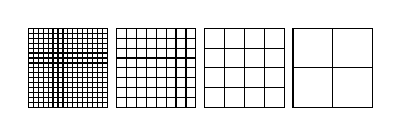
\begin{tikzpicture}
      [>=stealth,
      every node/.style={inner sep=2pt},
      restrict/.style={thick},
      prolong/.style={thick},
      mglevel/.style={rounded rectangle,draw=blue!50!black,fill=blue!20,thick,minimum size=4mm},
      ]
      \begin{scope}\scriptsize
        \newcommand\mgdx{4.0em}
        \newcommand\mgdy{4.0em}
        \newcommand\mgl[1]{(pow(2,#1+1))}
        \newcommand\mgloc[4]{(#1 + #4*\mgdx*#3,#2 + \mgdy*#3)}

        \newcommand\mghx{0.9*\mgdx}
        \newcommand\mghy{0.9*\mgdy}

        \draw[shift=\mgloc{0*\mgdx}{0}{0}{0},
        xstep=\mghy/\mgl{3},
        ystep=\mghy/\mgl{3}]
        (-0.5*\mghy,-0.5*\mghy) grid (0.5*\mghy,0.5*\mghy);

        \draw[shift=\mgloc{1*\mgdx}{0}{0}{0},
        xstep=\mghy/\mgl{2},
        ystep=\mghy/\mgl{2}]
        (-0.5*\mghy,-0.5*\mghy) grid (0.5*\mghy,0.5*\mghy);

        \draw[shift=\mgloc{2*\mgdx}{0}{0}{0},
        xstep=\mghy/\mgl{1},
        ystep=\mghy/\mgl{1}]
        (-0.5*\mghy,-0.5*\mghy) grid (0.5*\mghy,0.5*\mghy);


        \draw[shift=\mgloc{3*\mgdx}{0}{0}{0},
        xstep=\mghy/\mgl{0},
        ystep=\mghy/\mgl{0}]
        (-0.5*\mghy,-0.5*\mghy) grid (0.5*\mghy,0.5*\mghy);
      \end{scope}
    \end{tikzpicture}
    \label{fig:levels}
  \end{figure}
  \textbf{Multigrid} is an $O(n)$ method for solving algebraic problems by defining a hierarchy of scale.
  A multigrid method is constructed from:
  \begin{enumerate}
  \item a series of discretizations
    \begin{itemize}
    \item coarser approximations of the original problem
    \item constructed algebraically or geometrically
    \end{itemize}
  \item intergrid transfer operators
    \begin{itemize}
    \item residual restriction $I_h^H$ (fine to coarse)
    \item state restriction $\hat I_h^H$ (fine to coarse)
    \item partial state interpolation $I_H^h$ (coarse to fine, `prolongation')
    \item state reconstruction $\mathbb{I}_H^h$ (coarse to fine)
    \end{itemize}
  \item Smoothers ($S$)
    \begin{itemize}
    \item correct the high frequency error components
    \item Richardson, Jacobi, Gauss-Seidel, etc.
    \item Gauss-Seidel-Newton or optimization methods
    \end{itemize}
  \end{enumerate}
\end{frame}
\begin{frame}{$\tau$ formulation of Full Approximation Scheme (FAS)}
  \begin{itemize}
  \item classical formulation: ``coarse grid \emph{accelerates} fine grid solution''
  \item $\tau$ formulation: ``fine grid improves accuracy of coarse grid''
  \item To solve $N u = f$, recursively apply
    \begin{equation*}
      \begin{split}
        \text{pre-smooth} \:\: & \quad \tilde u^h \gets S^h_{\text{pre}}(u^h_0, f^h) \\
        \text{solve coarse problem for $u^H$} \:\: & \quad N^H u^H = f^H + \underbrace{N^H \hat I_h^H \tilde u^h - I_h^H N^h \tilde u^h}_{\tau_h^H} \\
        \text{correction and post-smooth} \:\: & \quad u^h \gets S^h_{\text{post}} \Big( \tilde u^h + I_H^h (u^H - \hat I_h^H \tilde u^h), f^h \Big) \\
      \end{split}
    \end{equation*}
    \begin{tabular}{ll}
      \toprule
      $I_h^H$ & residual restriction \\
      $\hat I_h^H$ & solution restriction \\
      $I_H^h$ & solution interpolation \\
      $f^H = I_h^H f^h$ & restriction of forcing term \\
      $\{S^h_{\text{pre}},S^h_{\text{post}}\}$ & smoothing operations on the fine grid \\
      \bottomrule
    \end{tabular}
  \end{itemize}
\end{frame}

\begin{frame}{Multiscale compression and recovery using $\tau$}
  % \begin{tikzpicture}
  %   [>=stealth,
  %   every node/.style={inner sep=2pt},
  %   restrict/.style={thick,double},
  %   prolong/.style={thick,double},
  %   cprestrict/.style={green!50!black,thick,double,dashed},
  %   control/.style={rectangle,red!40!black,draw=red!40!black,thick},
  %   mglevel/.style={rounded rectangle,draw=blue!50!black,fill=blue!20,thick,minimum size=4mm},
  %   checkpoint/.style={rectangle,draw=green!50!black,fill=green!20,thick,minimum size=4mm},
  %   mglevelhide/.style={rounded rectangle,draw=gray!50!black,fill=gray!20,thick,minimum size=4mm},
  %   tau/.style={text=red!50!black,draw=red!50!black,fill=red!10,inner sep=1pt}
  %   ]
  %   \begin{scope}\scriptsize
  %     \newcommand\mgdx{2.1em}
  %     \newcommand\mgdy{1.9em}
  %     \newcommand\mgloc[4]{(#1 + #4*\mgdx*#3,#2 + \mgdy*#3)}
  %     \node[mglevel] (fine0) at \mgloc{0}{0}{4}{-1} {\mglevelfine};
  %     \node[mglevel] (finem1down0) at \mgloc{0}{0}{3}{-1} {};
  %     \node[mglevel] (cp1down0) at \mgloc{0}{0}{2}{-1} {$\mglevelcp+1$};
  %     \node[mglevel] (cpdown0) at \mgloc{0}{0}{1}{-1} {\mglevelcp};
  %     \node[mglevel] (coarser0) at \mgloc{0}{0}{0}{0} {\ldots};

  %     \node[mglevelhide] (cpup0) at \mgloc{0}{0}{1}{1} {};
  %     \node (cp1up0) at \mgloc{0}{0}{2}{1} {};

  %     \node (cpdown1) at \mgloc{4em}{0}{1}{-1} {};
  %     \node[mglevelhide] (coarser1) at \mgloc{4em}{0}{0}{1} {\ldots};
  %     \node[mglevel] (cpup1) at \mgloc{4em}{0}{1}{1} {\mglevelcp};
  %     \node[mglevel] (cp1up1) at \mgloc{4em}{0}{2}{1} {$\mglevelcp+1$};
  %     \node[mglevel] (finem1up1) at \mgloc{4em}{0}{3}{1} {};
  %     \node[mglevel] (fine1) at \mgloc{4em}{0}{4}{1} {\mglevelfine};

  %     \draw[->,restrict,dashed] (fine0) -- (finem1down0);
  %     \draw[->,restrict] (finem1down0) -- (cp1down0);
  %     \draw[->,restrict] (cp1down0) -- (cpdown0);
  %     \draw[->,restrict,dashed] (cpdown0) -- (coarser0);
  %     \draw[->,prolong,dashed] (coarser0) -- (cpup0);
  %     \draw[->,prolong,dashed] (cpup0) -- (cp1up0);

  %     \draw[->,restrict,dashed] (cpdown1) -- (coarser1);
  %     \draw[->,prolong,dashed] (coarser1) -- (cpup1);
  %     \draw[->,prolong] (cpup1) -- (cp1up1);
  %     \draw[->,prolong] (cp1up1) -- (finem1up1);
  %     \draw[->,prolong,dashed] (finem1up1) -- (fine1);

  %     \node[checkpoint] at (4em + \mgdx*4,\mgdy) (cp) {CP};
  %     \draw[>->,cprestrict] (fine1) -- node[below,sloped] {Restrict} (cp);

  %     \node[left=\mgdx of fine0] (bnanchor) {};
  %     \node[control,fill=red!20] at (1.1*\mgdx,3*\mgdy) {Solve $F(u^n;b^n) = 0$};
  %     \node[mglevel,right=of fine1] (finedt) {next solve};
  %     \draw[->, >=stealth, control] (fine1) to[out=20,in=170] node[above] {$b^{n+1}(u^n,b^n)$} (finedt);
  %     \draw[->, >=stealth, control] (bnanchor) to[out=45,in=155] node[above] {$b^n$} (fine0);

  %     % Recovery process
  %     \begin{scope}[xshift=7*\mgdx]
  %       \node[checkpoint] (rcp) at \mgloc{0}{0}{0}{0} {CP};
  %       \node[mglevel] (r0a) at \mgloc{0}{\mgdy}{0}{0} {CR};
  %       \node[mglevel] (r1a) at \mgloc{0}{\mgdy}{1}{1} {};
  %       \node[mglevel] (r0b) at \mgloc{2*\mgdx}{\mgdy}{0}{0} {CR};
  %       \node[mglevel] (r1b) at \mgloc{2*\mgdx}{\mgdy}{1}{1} {};
  %       \node[mglevel] (r2b) at \mgloc{2*\mgdx}{\mgdy}{2}{1} {\mglevelfine};
  %       \node[mglevel] (r1c) at \mgloc{6*\mgdx}{\mgdy}{1}{-1} {};
  %       \node[mglevel] (r0d) at \mgloc{6*\mgdx}{\mgdy}{0}{0} {CR};
  %       \node[mglevel] (r1d) at \mgloc{6*\mgdx}{\mgdy}{1}{1} {};
  %       \node[mglevel] (r2d) at \mgloc{6*\mgdx}{\mgdy}{2}{1} {\mglevelfine};

  %       \draw[-,prolong,green!50!black] (rcp) -- (r0a);
  %       \draw[->,prolong] (r0a) -- (r1a);
  %       \draw[->,restrict] (r1a) -- (r0b);
  %       \draw[->,restrict] (r0b) -- (r1b);
  %       \draw[->,restrict,dashed] (r1b) -- (r2b);
  %       \draw[->,restrict,dashed] (r2b) -- (r1c);
  %       \draw[->,restrict] (r1c) -- (r0d);
  %       \draw[->,restrict] (r0d) -- (r1d);
  %       \draw[->,restrict,dashed] (r1d) -- (r2d);

  %       \foreach \smooth in {finem1down0, cp1down0, cpdown0, coarser0,
  %         cpup1, cp1up1, finem1up1,
  %         r0b,r1c,r0d,r1d} {
  %         \node[above left=-5pt of \smooth.west,tau] {$\tau$};
  %       }
  %       \node[rectangle,fill=none,draw=green!50!black,thick,fit=(rcp)(r2d)] (recoverbox) {};
  %       \node[rectangle,draw=green!50!black,fill=green!20,thick,minimum size=6mm,above={0cm of recoverbox.south east},anchor=south east] (recover) {FMG Recovery};
  %     \end{scope}
  %     \node (notation) at (-7.5*\mgdx,2*\mgdy) {
  %       \tiny
  %       \begin{minipage}{22em}\raggedright \sf
  %         $\bullet$ checkpoint converged coarse state \\
  %         $\bullet$ recover using FMG anchored at $\mglevelcp+1$ \\
  %         $\bullet$ compatible relaxation (CR) as coarse solve \\
  %         $\bullet$ $\tau$ correction is local, only $\mglevelcp$ neighbor points \\
  %         $\bullet$ survivors continue MG cycles with stale $\tau$
  %       \end{minipage}
  %     };
  %   \end{scope}
  % \end{tikzpicture}
  \includegraphics[width=\textwidth]{FMGRecovery}
    \begin{itemize}
    \item Compress transient simulation with local decompression
    \item Remove communication from all but coarse grid
      \begin{itemize}
      \item Convergence speed not affected, modest redundant computation
      \end{itemize}
    \item In-situ visualization and reanalysis with very few full checkpoints
    \item Checkpointing for discrete adjoints
    \item Resiliency to hardware failure
    \end{itemize}
\end{frame}


\begin{frame}{$\tau$ corrections}
  \begin{figure}
  \centering
  \begin{subfigure}[b]{0.18\textwidth}
    \includegraphics[width=\textwidth]{figures/MG/ElasticityCompressTrim}
    %\caption{Initial solution.}\label{fig:elast-initial}
  \end{subfigure} ~
  \begin{subfigure}[b]{0.18\textwidth}
    \includegraphics[width=\textwidth]{figures/MG/ElasticityCompressShearTrim}
    %\caption{Increment.}\label{fig:elast-increment}
  \end{subfigure} ~
  \begin{subfigure}[b]{0.28\textwidth}
    \includegraphics[width=\textwidth]{figures/MG/ElasticityCompressErrorNoTauTrim}
    %\caption{Smoothed error without $\tau$.}\label{fig:elast-error-notau}
  \end{subfigure} ~
  \begin{subfigure}[b]{0.28\textwidth}
    \includegraphics[width=\textwidth]{figures/MG/ElasticityCompressErrorTauTrim}
    %\caption{Smoothed error with $\tau$.}\label{fig:elast-error-tau}
  \end{subfigure}
  \begin{itemize}
  \item Plane strain elasticity, $E=1000,\nu=0.4$ inclusions in $E=1,\nu=0.2$ material, coarsen by $3^2$.
  \item Solve initial problem everywhere and compute $\tau_h^H = A^H \hat I_h^H u^h - I_h^H A^h u^h$
  \item Change boundary conditions and solve FAS coarse problem
    \begin{equation*}
      N^H \acute u^H = \underbrace{I_h^H \acute f^h}_{\acute f^H} + \underbrace{N^H \hat I_h^H \tilde u^h - I_h^H N^h \tilde u^h}_{\tau_h^H}
    \end{equation*}
  \item Prolong, post-smooth, compute error $e^h = \acute u^h - (N^h)^{-1} \acute f^h$
  \item<2> \alert{Coarse grid \emph{with $\tau$} is nearly $10\times$ better accuracy}
  \end{itemize}
  % \caption{Plane strain elasticity, $E=1000,\nu=0.4$ inclusions in $E=1,\nu=0.2$ material.  2-level multigrid with coarsening factor of $3^2$.
  %   Panes (a) and (b) show the deformed body colored by strain.
  %   The initial problem of compression by 0.2 from the right is solved (a) and $\tau = A^H \hat I_h^H u^h - I_h^H A^h u^h$ is computed.
  %   Then a shear increment of 0.1 in the $y$ direction is added to the boundary condition, and the coarse-level problem is resolved, interpolated to the fine-grid, and a post-smoother is applied.
  %   When the coarse problem is solved without a $\tau$ correction (c), the displacement error is nearly $10\times$ larger than when $\tau$ is included in the right hand side of the coarse problem (d).
  % }\label{fig:tau-valid}
  % ./ex49 -mx 90 -my 90 -da_refine_x 3 -da_refine_y 3 -elas_ksp_converged_reason -elas_ksp_rtol 1e-8 -no_view -c_str 3 -sponge_E0 1 -sponge_E1 1e3 -sponge_nu0 0.4 -sponge_nu1 0.2 -sponge_t 3 -sponge_w 9 -u_o vtk:ex49_sol.vts -use_nonsymbc -elas_pc_type mg -elas_pc_mg_levels 2 -elas_pc_mg_galerkin -tau1_o vtk:ex49_tau1.vts -tau2_o vtk:ex49_tau2.vts -taudiff_o vtk:ex49_taudiff.vts -u2_o vtk:ex49_sol2.vts -u2c_o vtk:ex49_sol2c.vts -u3_o vtk:ex49_sol3.vts -u4_o vtk:ex49_sol4.vts -u2err_o vtk:ex49_sol2err.vts -u3err_o vtk:ex49_sol3err.vts -u3c_o vtk:ex49_sol3c.vts -tau3_o vtk:ex49_tau3.vts
\end{figure}
\end{frame}

\begin{frame}{$\tau$ adaptivity for heterogeneous media}
  \begin{itemize}
  \item Applications
    \begin{itemize}
    \item Geo: reservoir engineering, lithosphere dynamics (subduction, rupture/fault dynamics)
    \item carbon fiber, biological tissues, fracture
    \item Conventional adaptivity fails
    \end{itemize}
  \item Traditional adaptive methods fail
    \begin{itemize}
    \item Solutions are not ``smooth''
    \item Cannot build accurate coarse space without scale separation
    \end{itemize}
  \item $\tau$ adaptivity
    \begin{itemize}
    \item Fine-grid work needed everywhere at first
    \item Then $\tau$ becomes accurate in nearly-linear regions
    \item Only visit fine grids in ``interesting'' places: active nonlinearity, drastic change of solution
    \end{itemize}
  \end{itemize}
\end{frame}

\begin{frame}{Comparison to nonlinear domain decomposition}
  \begin{itemize}
  \item ASPIN (Additive Schwarz preconditioned inexact Newton) \\
    \begin{itemize}
    \item Cai and Keyes (2003)
    \item More local iterations in strongly nonlinear regions
    \item Each nonlinear iteration only propagates information locally
    \item Many real nonlinearities are activated by long-range forces
      \begin{itemize}
      \item locking in granular media (gravel, granola)
      \item binding in steel fittings, crack propagation
      \end{itemize}
    \item Two-stage algorithm has different load balancing
      \begin{itemize}
      \item Nonlinear subdomain solves
      \item Global linear solve
      \end{itemize}
    \end{itemize}
  \item $\tau$ adaptivity
    \begin{itemize}
    \item Minimum effort to communicate long-range information
    \item Nonlinearity sees effects as accurate as with global fine-grid feedback
    \item Fine-grid work always proportional to ``interesting'' changes
    \end{itemize}
  \end{itemize}
\end{frame}

\subsection{Reducing communication and memory bandwidth}
\begin{frame}{Low communication MG}
  \begin{columns}
    \begin{column}{0.55\textwidth}
      \begin{itemize}
      \item {\color{red} red arrows} can be removed by $\tau$-FAS with overlap
      \item {\color{blue} blue arrows} can also be removed, but then
        algebraic convergence stalls when discretization error is
        reached
      \item no simple way to check that discretization error is obtained
      \item if fine grid state is not stored, use compatible relaxation to complete prolongation $P$
      \end{itemize}
    \end{column}
    \begin{column}{0.45\textwidth}
      \vspace{-2em}
      \includegraphics[width=\textwidth]{figures/MG/LowCommunication}
    \end{column}
  \end{columns}
\end{frame}

\begin{frame}{Reducing memory bandwidth}
  \includegraphics[width=\textwidth]{figures/MG/SRMGWindow}
  \begin{itemize}
  \item Sweep through ``coarse'' grid with moving window
  \item Zoom in on new slab, construct fine grid ``window'' in-cache
  \item Interpolate to new fine grid, apply pipelined smoother ($s$-step)
  \item Compute residual, accumulate restriction of state and residual into coarse grid, expire slab from window
  \end{itemize}
\end{frame}

\begin{frame}{Arithmetic intensity of sweeping visit}
  \begin{itemize}
  \item Assume 3D cell-centered, 7-point stencil
  \item 14 flops/cell for second order interpolation
  \item $\ge 15$ flops/cell for fine-grid residual or point smoother
  \item 2 flops/cell to enforce coarse-grid compatibility
  \item 2 flops/cell for plane restriction
  \item assume coarse grid points are reused in cache
  \item Fused visit reads $u^H$ and writes $\hat I_h^H u^h$ and $I_h^H r^h$
  \item Arithmetic Intensity
    \begin{equation}
      \frac{{\overbrace{15}^{\text{interp}}} + {\overbrace{2\cdot (15+2)}^{\text{compatible relaxation}}} + \overbrace{2\cdot 15}^{\text{smooth}} + \overbrace{15}^{\text{residual}} + \overbrace{2}^{\text{restrict}}}{3 \cdot \texttt{sizeof(scalar)} / \underbrace{2^3}_{\text{coarsening}}} \gtrsim 30
    \end{equation}
  \item Still $\gtrsim 10$ with non-compressible fine-grid forcing
  \end{itemize}
\end{frame}

\begin{frame}{Regularity}
  Accuracy of recovery depends on operator regularity
  \begin{itemize}
  \item Even with regularity, we can only converge up to discretization error, unless we add a \emph{consistent} fine-grid residual evaluation
  \item Visit fine grid with some overlap, but patches do not agree exactly in overlap
  \item Need decay length for high-frequency error components (those that restrict to zero) that is bounded with respect to grid size
  \item Required overlap $J$ is proportional to the number of cells to cover decay length
  \item Can enrich coarse space along boundary, but causes loss of coarse-grid sparsity
  \item Brandt and Diskin (1994) has two-grid LFA showing $J \lesssim 2$ is sufficient for Laplacian
  \item With $L$ levels, overlap $J(k)$ on level $k$,
    \begin{equation*}
      2J(k) \ge s (L-k+1)
    \end{equation*}
    where $s$ is the smoothness order of the solution or the discretization order (whichever is smaller)
  \end{itemize}
\end{frame}

\subsection{Local recovery and postprocessing}
\begin{frame}{Basic resilience strategy}
  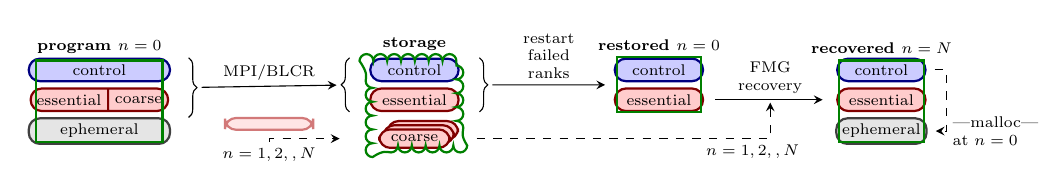
\begin{tikzpicture}
    [scale=0.8,every node/.style={scale=0.8},
    >=stealth,
    control/.style={rectangle,rounded corners,draw=blue!50!black,fill=blue!20,thick,minimum width=5em},
    essential/.style={rectangle,rounded corners,draw=red!50!black,fill=red!20,thick,minimum width=5em},
    ephemeral/.style={rectangle,rounded corners,draw=gray!50!black,fill=gray!20,thick,minimum width=5em},
    statebox/.style={rectangle,draw=green!50!black,thick},
    statetitle/.style={rectangle,draw=green!50!black,fill=green!20,thick},
    storebox/.style={rectangle,draw=},
    rightbrace/.style={decorate,decoration={brace,amplitude=1ex,raise=4pt}},
    leftbrace/.style={decorate,decoration={brace,amplitude=1ex,raise=4pt,mirror}}
    ]
    \scriptsize
    \node[control,minimum width=8em] (progcontrol) {control};
    \node[essential,below=2pt of progcontrol.south,rectangle split,rectangle split parts=2,rectangle split horizontal,minimum width=12em] (progessential) {essential \nodepart{two} coarse};
    \node[ephemeral,minimum width=8em,below=2pt of progessential.south] (progephemeral) {ephemeral};
    \node[statebox,fit=(progcontrol)(progessential)(progephemeral)] (progbox) {};
    \node[above=0pt of progbox.north,anchor=south] {\textbf{program $n=0$}};

    \node[control,right=9em of progcontrol] (storecontrol) {control};
    \node[essential,below=2pt of storecontrol.south] (storeessential) {essential};
    \node[essential,minimum width=4em,below=6pt of storeessential.south, double copy shadow] (storecoarse) {coarse};
    \node[statebox,decorate,decoration={bumps,mirror},fit=(storecontrol)(storecoarse)] (storebox) {};
    \node[above=1pt of storebox.north,anchor=south] {\textbf{storage}};

    \node[control,right=7em of storecontrol] (reccontrol) {control};
    \node[essential,below=2pt of reccontrol.south] (recessential) {essential};
    \node[statebox,fit=(reccontrol)(recessential)] (recbox) {};
    \node[above=0pt of recbox.north,anchor=south] {\textbf{restored $n=0$}};

    \node[control,right=6em of reccontrol] (donecontrol) {control};
    \node[essential,below=2pt of donecontrol.south] (doneessential) {essential};
    \node[ephemeral,below=2pt of doneessential.south] (doneephemeral) {ephemeral};
    \node[statebox,fit=(donecontrol)(doneephemeral)] (donebox) {};
    \node[above=0pt of donebox.north,anchor=south] {\textbf{recovered $n=N$}};

    \draw[decorate,decoration={brace,amplitude=1ex,raise=4pt}] ($(progcontrol.north east) + (3pt,0)$) -- ($(progephemeral.north east) + (3pt,0)$) node[midway,xshift=1ex] (progbrace) {};
    \draw[leftbrace] ($(storecontrol.north west) - (4pt,0)$) -- ($(storeessential.south west) - (4pt,0)$) node[midway,xshift=-1ex] (storebrace) {};
    \draw[rightbrace] ($(storecontrol.north east) + (4pt,0)$) -- ($(storeessential.south east) + (4pt,0)$) node[midway,xshift=1ex] (storerbrace) {};
    \draw[->,shorten >=4pt,shorten <=4pt] (progbrace) -- (storebrace) node[midway,above] (midarrow) {MPI/BLCR};

    \node[below=1.4em of midarrow,essential,draw=red!50!gray!70,fill=red!10] (coarserun) {};
    \draw[->,dashed,shorten >=14pt,shorten <=4pt] (coarserun) |- (storecoarse) node [near start,below,yshift=-3pt] {\scriptsize $n=1,2,\dotsc,N$};
    \draw[->,shorten >=4pt,shorten <=4pt] (storerbrace) -- (recbox.west) node[midway,above,text width=5em,align=center] (midarrow) {restart failed ranks};
    \draw[->,shorten >=5pt,shorten <=4pt] (recessential.east) -- (doneessential) node[midway,above,text width=5em,align=center] (fmgrecover) {FMG recovery};
    \draw[->,dashed,shorten >=1pt,shorten <=3pt] ($(storecoarse.east) + (1em,0)$) -| (fmgrecover) node[midway,below,xshift=-1em] {\scriptsize $n=1,2,\dotsc,N$};
    \draw[->,dashed,shorten >=3pt,shorten <=3pt] (donecontrol.east) -| ($(donecontrol.east) + (3ex,0)$) |- (doneephemeral.east) node[midway,right,text width=4em] {\cverb|malloc| at $n=0$};
  \end{tikzpicture}
\begin{description}
\item[control] contains program stack, solver configuration, etc.
\item[essential] program state that cannot be easily reconstructed: time-dependent solution, current optimization/bifurcation iterate
\item[ephemeral] easily recovered structures: assembled matrices, preconditioners, residuals, Runge-Kutta stage solutions
\end{description}
\begin{itemize}
\item Essential state at time/optimization step $n$ is \alert{inherently globally coupled} to step $n-1$ (otherwise we could use an explicit method)
\item \emph{Coarse} level checkpoints are orders of magnitude smaller, but allow rapid recovery of essential state
\item FMG recovery needs only \alert{nearest neighbors}
\end{itemize}
\end{frame}

\begin{frame}[fragile]{Multiscale compression and recovery using $\tau$ form}
   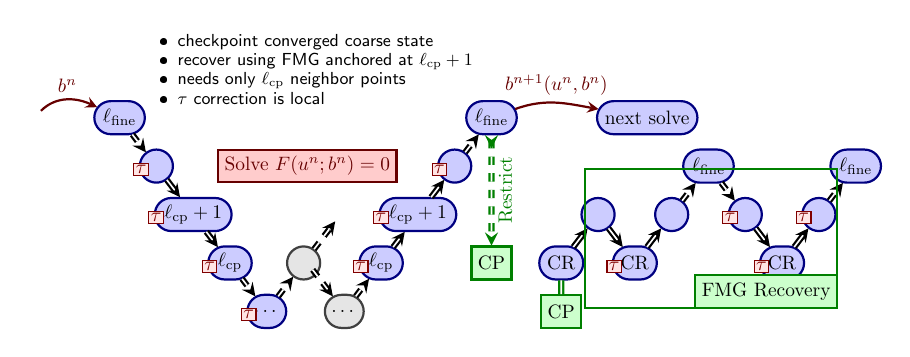
\begin{tikzpicture}
    [scale=0.7,every node/.style={scale=0.7},
    >=stealth,
    restrict/.style={thick,double},
    prolong/.style={thick,double},
    cprestrict/.style={green!50!black,thick,double,dashed},
    control/.style={rectangle,red!40!black,draw=red!40!black,thick},
    mglevel/.style={rounded rectangle,draw=blue!50!black,fill=blue!20,thick,minimum size=6mm},
    checkpoint/.style={rectangle,draw=green!50!black,fill=green!20,thick,minimum size=6mm},
    mglevelhide/.style={rounded rectangle,draw=gray!50!black,fill=gray!20,thick,minimum size=6mm},
    tau/.style={text=red!50!black,draw=red!50!black,fill=red!10,inner sep=1pt},
    crelax/.style={text=green!50!black,fill=green!10,inner sep=0pt}
    ]
    \begin{scope}
      \newcommand\mgdx{1.9em}
      \newcommand\mgdy{2.5em}
      \newcommand\mgloc[4]{(#1 + #4*\mgdx*#3,#2 + \mgdy*#3)}
      \node[mglevel] (fine0) at \mgloc{0}{0}{4}{-1} {\mglevelfine};
      \node[mglevel] (finem1down0) at \mgloc{0}{0}{3}{-1} {};
      \node[mglevel] (cp1down0) at \mgloc{0}{0}{2}{-1} {$\mglevelcp+1$};
      \node[mglevel] (cpdown0) at \mgloc{0}{0}{1}{-1} {\mglevelcp};
      \node[mglevel] (coarser0) at \mgloc{0}{0}{0}{0} {\ldots};

      \node[mglevelhide] (cpup0) at \mgloc{0}{0}{1}{1} {};
      \node (cp1up0) at \mgloc{0}{0}{2}{1} {};

      \node (cpdown1) at \mgloc{4em}{0}{1}{-1} {};
      \node[mglevelhide] (coarser1) at \mgloc{4em}{0}{0}{1} {\ldots};
      \node[mglevel] (cpup1) at \mgloc{4em}{0}{1}{1} {\mglevelcp};
      \node[mglevel] (cp1up1) at \mgloc{4em}{0}{2}{1} {$\mglevelcp+1$};
      \node[mglevel] (finem1up1) at \mgloc{4em}{0}{3}{1} {};
      \node[mglevel] (fine1) at \mgloc{4em}{0}{4}{1} {\mglevelfine};

      \draw[->,restrict,dashed] (fine0) -- (finem1down0);
      \draw[->,restrict] (finem1down0) -- (cp1down0);
      \draw[->,restrict] (cp1down0) -- (cpdown0);
      \draw[->,restrict,dashed] (cpdown0) -- (coarser0);
      \draw[->,prolong,dashed] (coarser0) -- (cpup0);
      \draw[->,prolong,dashed] (cpup0) -- (cp1up0);

      \draw[->,restrict,dashed] (cpdown1) -- (coarser1);
      \draw[->,prolong,dashed] (coarser1) -- (cpup1);
      \draw[->,prolong] (cpup1) -- (cp1up1);
      \draw[->,prolong] (cp1up1) -- (finem1up1);
      \draw[->,prolong,dashed] (finem1up1) -- (fine1);

      \node[checkpoint] at (4em + \mgdx*4,\mgdy) (cp) {CP};
      \draw[>->,cprestrict] (fine1) -- node[below,sloped] {Restrict} (cp);

      \node[left=\mgdx of fine0] (bnanchor) {};
      \node[control,fill=red!20] at (1.1*\mgdx,3*\mgdy) {Solve $F(u^n;b^n) = 0$};
      \node[mglevel,right=of fine1] (finedt) {next solve};
      \draw[->, >=stealth, control] (fine1) to[out=20,in=170] node[above] {$b^{n+1}(u^n,b^n)$} (finedt);
      \draw[->, >=stealth, control] (bnanchor) to[out=45,in=155] node[above] {$b^n$} (fine0);

      % Recovery process
      \begin{scope}[xshift=8*\mgdx]
        \node[checkpoint] (rcp) at \mgloc{0}{0}{0}{0} {CP};
        \node[mglevel] (r0a) at \mgloc{0}{\mgdy}{0}{0} {CR};
        \node[mglevel] (r1a) at \mgloc{0}{\mgdy}{1}{1} {};
        \node[mglevel] (r0b) at \mgloc{2*\mgdx}{\mgdy}{0}{0} {CR};
        \node[mglevel] (r1b) at \mgloc{2*\mgdx}{\mgdy}{1}{1} {};
        \node[mglevel] (r2b) at \mgloc{2*\mgdx}{\mgdy}{2}{1} {\mglevelfine};
        \node[mglevel] (r1c) at \mgloc{6*\mgdx}{\mgdy}{1}{-1} {};
        \node[mglevel] (r0d) at \mgloc{6*\mgdx}{\mgdy}{0}{0} {CR};
        \node[mglevel] (r1d) at \mgloc{6*\mgdx}{\mgdy}{1}{1} {};
        \node[mglevel] (r2d) at \mgloc{6*\mgdx}{\mgdy}{2}{1} {\mglevelfine};

        \draw[-,prolong,green!50!black] (rcp) -- (r0a);
        \draw[->,prolong] (r0a) -- (r1a);
        \draw[->,restrict] (r1a) -- (r0b);
        \draw[->,restrict] (r0b) -- (r1b);
        \draw[->,restrict,dashed] (r1b) -- (r2b);
        \draw[->,restrict,dashed] (r2b) -- (r1c);
        \draw[->,restrict] (r1c) -- (r0d);
        \draw[->,restrict] (r0d) -- (r1d);
        \draw[->,restrict,dashed] (r1d) -- (r2d);

        \foreach \smooth in {finem1down0, cp1down0, cpdown0, coarser0,
          cpup1, cp1up1, finem1up1,
          r0b,r1c,r0d,r1d} {
          \node[above left=-5pt of \smooth.west,tau] {$\tau$};
        }
        \node[rectangle,fill=none,draw=green!50!black,thick,fit=(rcp)(r2d)] (recoverbox) {};
        \node[rectangle,draw=green!50!black,fill=green!20,thick,minimum size=6mm,above={0cm of recoverbox.south east},anchor=south east] (recover) {FMG Recovery};
      \end{scope}
      \node (notation) at (\mgdx,5*\mgdy) {
        \begin{minipage}{18em}\small\sf
          \begin{itemize}\addtolength{\itemsep}{-5pt}
          \item checkpoint converged coarse state
          \item recover using FMG anchored at $\mglevelcp+1$
          \item needs only $\mglevelcp$ neighbor points
          \item $\tau$ correction is local
          \end{itemize}
        \end{minipage}
      };
    \end{scope}
  \end{tikzpicture}
  \begin{itemize}
  \item Normal multigrid cycles visit all levels moving from $n \to n+1$
  \item FMG recovery only accesses levels finer than $\ell_{CP}$
  \item Only failed processes and neighbors participate in recovery
  \item Lightweight checkpointing for transient adjoint computation
  \item Postprocessing applications, e.g., in-situ visualization at high temporal resolution in part of the domain
  \end{itemize}
\end{frame}

\begin{frame}{First-order cost model for FAS resilience}
  Extend first-order locality-unaware model of Young (1974):
  \begin{description}
  \item[$\timeW$] time to write a heavy fine-grid checkpointed state
  \item[$\timeR$] time to read back lost state
  \item[$R$] fraction of forward simulation needed for recomputation from a saved state
  \item[$P$] the heavy checkpoint interval
  \item[$M$] mean time to failure
  \end{description}
  Neglect cost of I/O for lightweight coarse-grid checkpoints
  \begin{equation*}\label{eq:overhead}
    \text{Overhead} = 1 - \text{AppUtilization} = \underbrace{\frac{\timeW}{P}}_{\text{writing}}
    + \underbrace{\frac{\timeR}{M}}_{\text{reading after failure}}
    + \underbrace{\frac{R P}{2M}}_{\text{recomputation}}
  \end{equation*}
  Minimized for a heavy checkpointing interval $P = \sqrt{2 M \timeW / R}$
  \begin{equation*}\label{eq:minoverhead}
    \text{Overhead}^* = \sqrt{2 \timeW R / M} + \timeR / M
    % $ \text{Overhead}^* = \sqrt{\frac{2 \timeW R}{M}} + \frac{\timeR}{M} $,
  \end{equation*}
  where the first term is always larger than the second.
  Conventional checkpointing schemes store only fine-grid state, thus $R=1$ (recovery costs the same as initial computation).
\end{frame}


\begin{frame}{Outlook}
  \begin{itemize}
  \item Implicit Runge-Kutta
    \begin{itemize}
  \item Working: Tensor product matrices (TAIJ format) and one-level methods
  \item Next up: Algebraic multigrid for tensor product operators
  \item Research: imaginary rotation in coarse operators (cf. MG for Helmholtz)
  \item Stochastic Galerkin has same structure
  \item Is it possible to design methods with well-conditioned $S = X \Lambda X^{-1}$
    \end{itemize}
  \item $\tau$-adaptivity
    \begin{itemize}
    \item nonlinear smoothers (and discretizations)
    \item dynamic load balancing
    \item reliability of error estimates for refreshing $\tau$
    \end{itemize}
  \end{itemize}
\end{frame}

\end{document}
